\documentclass[a4paper, 10pt, conference]{ieeeconf}

\usepackage[dvipsnames]{xcolor}

\usepackage{times}
\usepackage{graphicx}
\usepackage{amssymb}
\usepackage{amsmath}
\usepackage{breakurl}
\def\UrlBreaks{\do\/\do-}
\usepackage{url,hyperref}
\usepackage{algorithm}
\usepackage{algorithmic}
\usepackage[labelfont={bf},font=small]{caption}
\usepackage[none]{hyphenat}
\usepackage{mathtools, cuted}
\usepackage[noadjust, nobreak]{cite}
\usepackage{tabularx}
\newcolumntype{Y}{>{\centering\arraybackslash}X}
\usepackage{afterpage}
\usepackage{stfloats}
\usepackage{comment}


\title{\LARGE \bf
Rubin Observatory Science Pipelines on AWS
}

\author{
    Dino Bektesevic$^1$, Andrew Connolly$^1$ \\
    Department of Astronomy, University of Washington \\ Email: dinob@uw.edu, ajc@uw.edu
    }

\begin{document}


\maketitle


%%%%%%%%%%%%%%%%%%%%%%%%%%%%%%%%%%%%%%%%%%%%%%%%%%%%%%%%%%%%%%%%%%%%%%%%%%%%%%%%
\begin{abstract}

The Legacy Survey of Space and Time\footnote{\url{www.lsst.org}} (LSST) aims to conduct a longitudinal 10 year long survey in which the entire night sky will be imaged every three nights. It is estimated LSST will produce 20TB of data per night and that, in the 10 years of operations it will deliver a total of 500 petabytes (PB) of data. In this paper we claim that the, pervasive in field of astronomy, subset-download-process paradigm of data reprocessing faces significant challenges at LSST data volumes and present the first comprehensive attempt at enabling astronomical image data reduction in the cloud. We focus on executing LSST's Science Pipelines, a collection of image and catalog processing algorithms, on Amazon Web Services (AWS). We describe how we utilize Pegasus Workflow Management System\footnote{\url{https://pegasus.isi.edu}} to describe, plan and execute a data processing pipeline and how we manage computing resources via HTCondor\footnote{\url{https://research.cs.wisc.edu/htcondor/}}. We discuss performance, scalability and cost of deploying on AWS.
\end{abstract}

%%%%%%%%%%%%%%%%%%%%%%%%%%%%%%%%%%%%%%%%%%%%%%%%%%%%%%%%%%%%%%%%%%%%%%%%%%%%%%%%
\section{INTRODUCTION}

Cloud computing has been widely utilized by the IT industry, however, its adoption by the Astronomy community has been slow. Currently pervasive model of sub-selecting, transferring to local compute resources and then reprocessing data are successful in context of past sky-surveys such as such as Sloan Digital Sky Survey\cite{York2000} (SDSS) because technological developments and pricing made acquiring sufficient local compute resource affordable. The new generation sky surveys, such as LSST, promise to deliver an order of magnitude more data rendering the subset-download-process paradigm unviable in the long-term. 

Drawing on lessons learned from previous surveys and in order to facilitate scientific discovery LSST reduces the raw data into multiple different, smaller in volume, science products. LSST also offers 10\% of their compute resources for use to in-collaboration scientists. Even though this approach mitigates a lot of associated problems it does not do away with the need to process pixel level data. On face value it would at least guarantee repeatability and reproducibility. At LSST's data volumes however, considering even a relatively small subset of data will amount to a large dataset, f.e. over the lifetime of the survey a 1\% random subset of the total data still constitutes a 5 PB large dataset. To reprocess even such small subsets of total data, significant computing resources, and subsequently significant initial investments, would be required.

Resorting to cloud computing alleviates both the issues of cost as well as scalability. Additionally it provides astronomers an easier access to state of the art astronomical data processing algorithms capable of reducing raw data from multiple different currently used instruments such as Dark Energy Camera (DECam), Hyper-Suprime Cam (HSC), SDSS and Canada-France-Hawaii Telescope (CFHT). Due to the design of LSST's Science Pipelines it is possible to alter, supplement or completely replace the data processing algorithms, thus enabling scientific validation and increasing the potential of scientific discovery.  


%%%%%%%%%%%%%%%%%%%%%%%%%%%%%%%%%%%%%%%%%%%%%%%%%%%%%%%%%%%%%%%%%%%%%%%%%%%%%%%%
\section{Technology Stack}

* some generic overview of how stack (scipipe and middleware) + pegasus + htcondor works

\begin{figure}[htb]
\centering
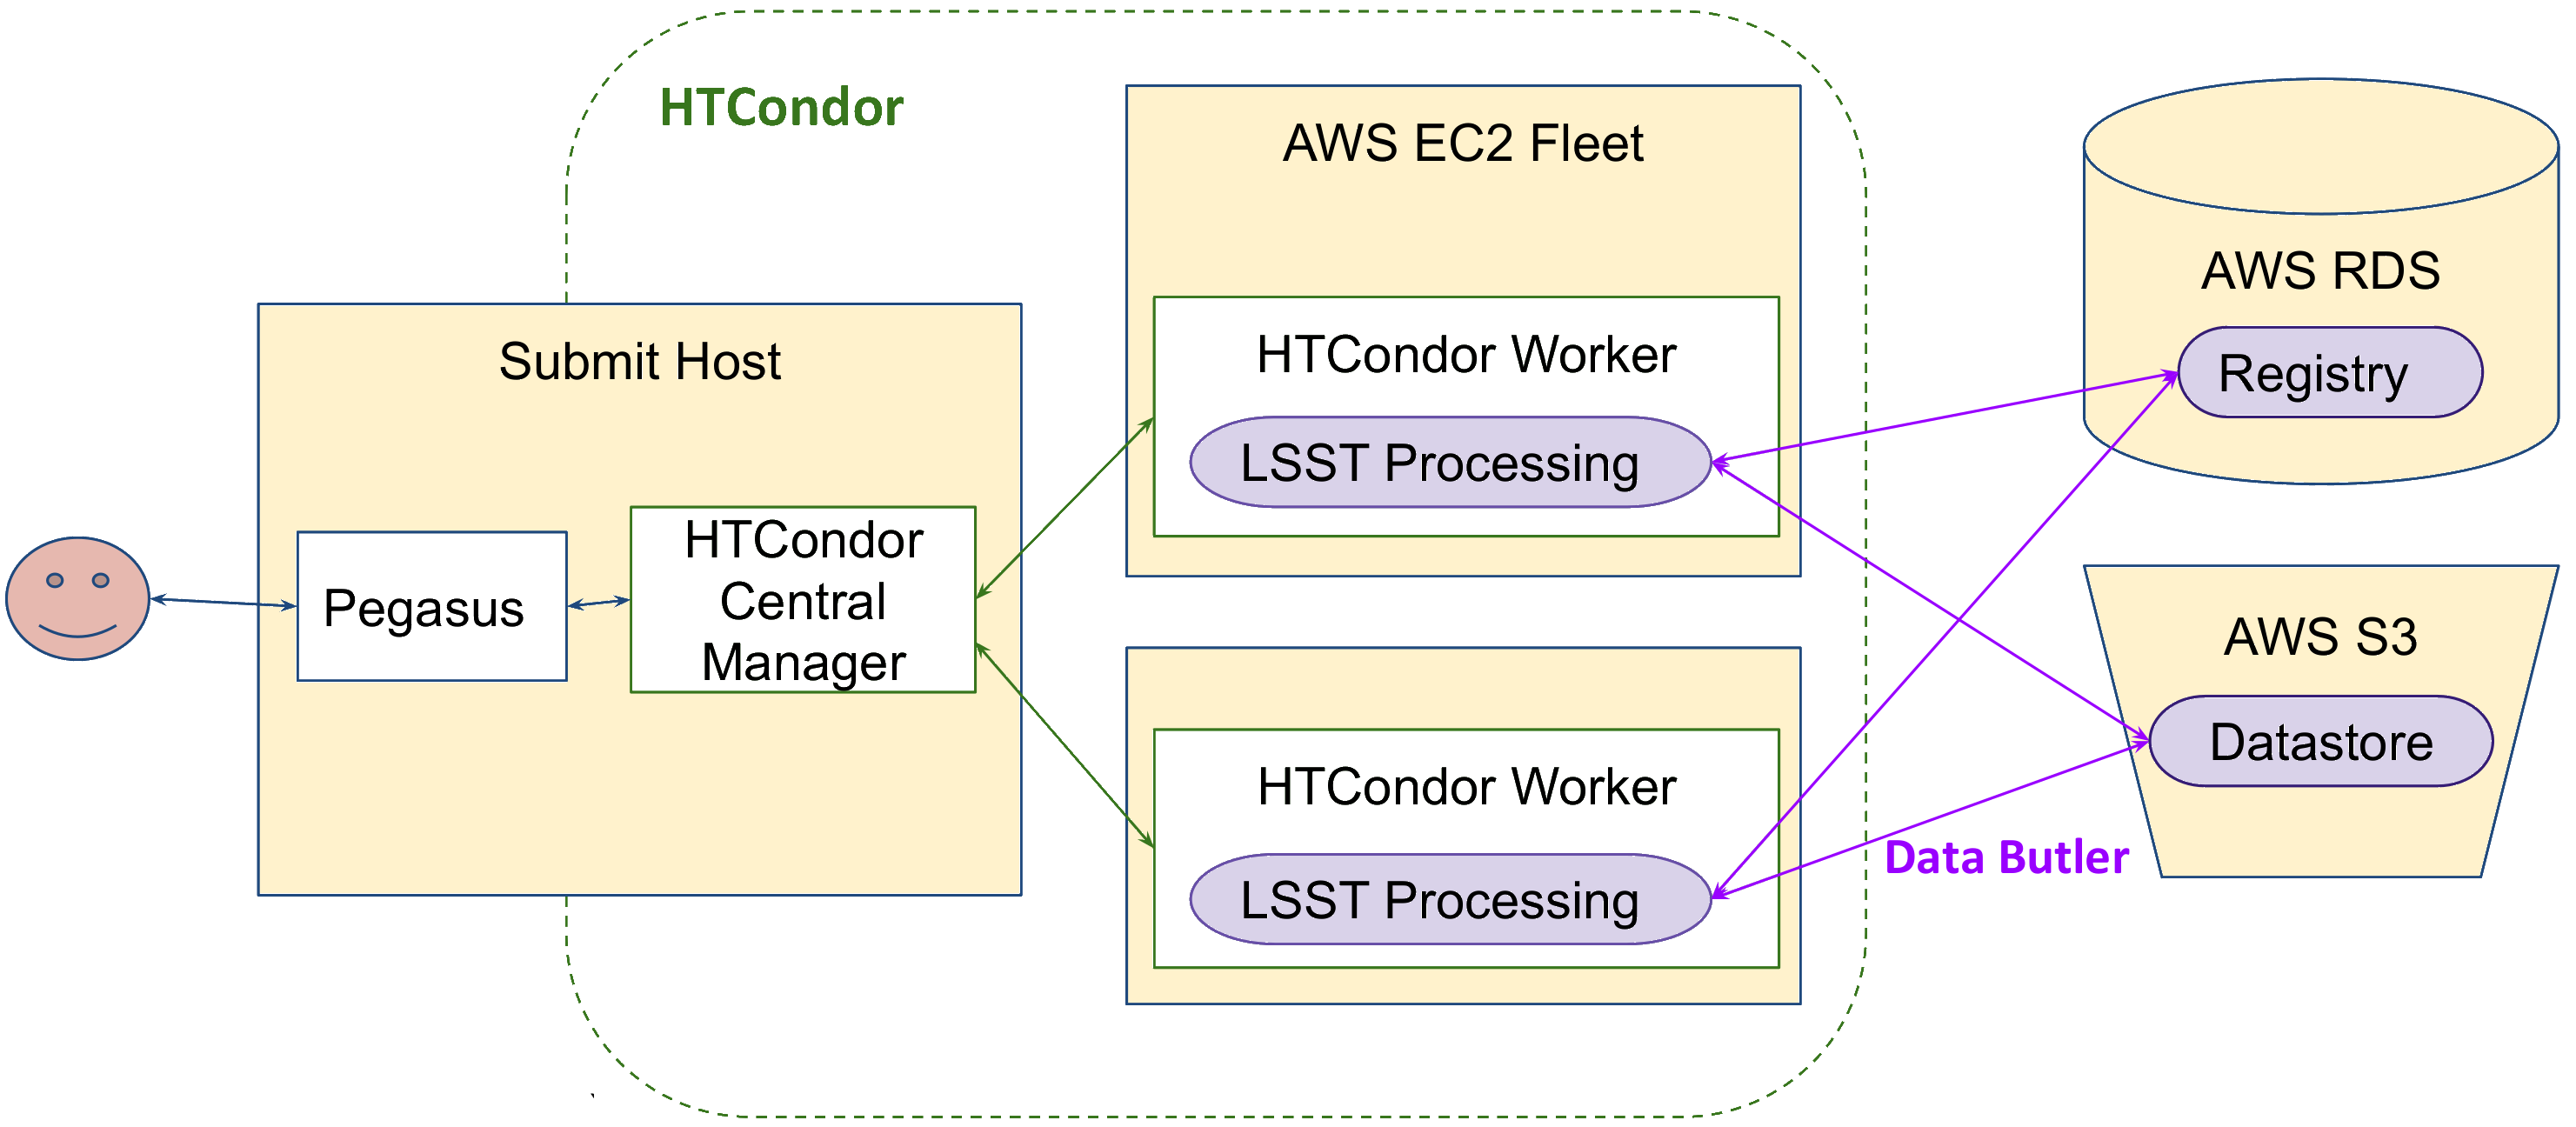
\includegraphics[width=\columnwidth]{figures/workflow.png}
\caption{Diagram of the Technology stack showing its components.}
\label{fig:techstack}
\end{figure}

\subsection{Science Pipelines and Middleware}

Science pipelines represent state of the art in astronomical data reduction. They consist of variety of configurable Tasks that can be chained into a pipeline. Such pipeline is described by a directed acyclic graph (DAG) called a QuantumGraph. Quantum Graph consists of quanta, which is a task applied {\color{red}to a singular dataset. REPHRASE BETTER}. Science Pipelines enable processing of optical and near-infrared astronomical data from a single visit (instrument signature removal, characterization, calibration, coaddition, forced photometry etc) to overarching tasks such as joint calibration that constrains astrometric and photometric measurements across multiple different visits. 

Tasks themselves are agnostic to the used file formats and locations of the data. The input-output (IO) and provenance is tracked through a middleware component called the Data Butler. The main purpose of the Data Butler is to isolate the end user from file organization, filetypes and related file access mechanisms by exposing datasets as, mostly, Python objects. Datasets are referred to by their unique IDs, or a set of identifying references. Data Butler uses an Registry to resolve the dataset references and resolves the location, file format and the Python object/type the files stored in a Datastore are to be read as.

The Registry is almost always backed by an SQL database and the Datastore is usually backed by a shared filesystem. Significant amount of work in this paper was the implementation of a Registry and a Datastore capable of utilizing AWS resources and is described in detail at \url{https://dmtn-114.lsst.io/} and \url{https://dmtn-137.lsst.io/} {\color{red} HOT TO CITE DMTNs?}

\subsection{Pegasus WMS and HTCondor}

\href{https://research.cs.wisc.edu/htcondor}{HTCondor} \cite{Thain:2005:HTCondor} provides distributed job parallelization and is a powerful batch system for high throughput computing (HTC). A HTCondor pool is a collection of compute resources, and HTCondor matches job requests with available resources following their job requirements. HTCondor Annex allows HTCondor deployment on cloud resources via acquisition of cloud compute resources external to an existing HTCondor pool. A pool can have multiple annexes, and each annex manages its own lifecycle. Unused compute resources are automatically deallocated after a user-set time spent idling. 

\href{https://pegasus.isi.edu/}{Pegasus} \cite{Deelman:2015:Pegasus} is a workflow management system built on top of HTCondor.
It provides command line and API interfaces for scientists to write an abstract workflow independent of the underlying computing infrastructure. Pegasus workflows are expressed as DAGs and Quantum Graphs are interpretable by Pegasus. Pegasus comes with various tools for data management, f.e. log transfers, and supports different execution strategies by grouping jobs within or across nodes of a DAG.


\subsection{Amazon Web Services}

Datastore implements \href{https://aws.amazon.com/s3/}{Simple Storage Service (S3)} as a backend. S3 is an object storage that allows massive amounts of unstructured data, where each object typically is identified by a globally unique identifier, to be stored and accessed in a durable and highly scalable way.

\href{https://aws.amazon.com/rds/}{Relational Database Service (RDS)} is the AWS cloud service that launches and configures databases with ease. PostgreSQL was chosen as the DBMS backend for the Registry. Primary drivers behind PostgreSQL were the ease of deploying in RDS, the common use of PostgreSQL as a Virtual Observatory (VO) Table Access Protocol (TAP) backend, no additional licensing fees usually associated with proprietary software and PostgreSQL's off-the-shelf support for spatial primitives needed for astronomy. The RDS databases can be backed up into snapshots as well as exported to downloadable files on S3.

Elastic Compute Cloud (EC2) is used to acquire compute resources.  EC2 service uses virtualization technology to deliver a variety of different pre-configured instance types optimized for different use cases. Within each instance type there are several different instance sizes comprised of varying combinations of CPU, memory, storage, and networking capacity. Amazon Machine Image (AMI) provides the information required to launch an instance and we provide pre-built CentOS AMIs that contain and configure the required parts of the technology stack fo both master and the workers. 
%%%%%%%%%%%%%%%%%%%%%%%%%%%%%%%%%%%%%%%%%%%%%%%%%%%%%%%%%%%%%%%%%%%%%%%%%%%%%%%%
\section{Example Workflow}

The example workflow is based off of the well understood, well characterized HSC Release Candidate dataset\footnote{\url{https://jira.lsstcorp.org/browse/DM-11345}}. This dataset is reprocessed using Rubin Obs. compute resources every two weeks in order to characterize the scientific validity and performance of the algorithms as they are being developed. The workflow consists of initialization, instrument signature removal, characterization and calibration jobs. Initialization job is responsible for correctly setting up metadata in the Registry. There are 6787 instrument signature removal (ISR) jobs. ISR removes image features that are the results of instrument flaws. Characterization consists of modeling the background, point spread function (PSF), repairing cosmic ray traces, detecting and measuring bright sources and measuring aperture correction. There are, again, 6787 characterize tasks in the workflow. Finally the calibration tasks, using PSF and aperture correction from previous step, detect all sources on the image and perform astrometry and photometry on the image. The workflow is shown on \ref{fig:demo-workflow}

\begin{figure}[htb]
\centering
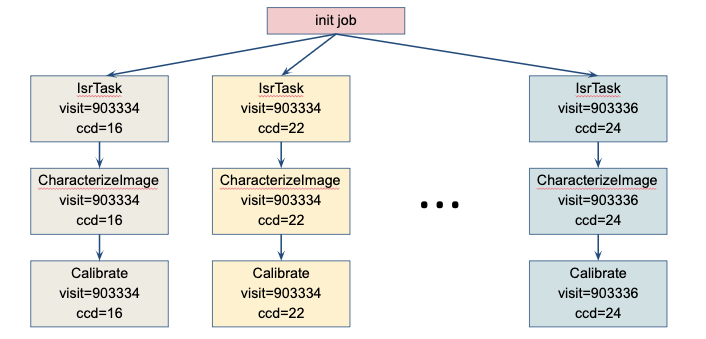
\includegraphics[width=\columnwidth]{figures/demo-workflow.png}
\caption{Example workflow on which performance and scalability was tested.}
\label{fig:demo-workflow}
\end{figure}

The total size of the output data is approximately 2TB. The dataset represents approximately 10\% of LSST's nightly data volume. 

maybe a nice figure of input, raw vs output calibrated exp (in progress)

\section{Performance, scalability and cost}
 - runs in an hour
 
 - costs 6\$
 
 - andy should really pay me more

%%%%%%%%%%%%%%%%%%%%%%%%%%%%%%%%%%%%%%%%%%%%%%%%%%%%%%%%%%%%%%%%%%%%%%%%%%%%%%%%
\section{Discussion}
- being optimal, or even comparable to LSST performance, is very difficult for general graphs because characterizing resource requirements is difficult

- bandwidth is really not a problem because distributive properties of S3

- there are, as of yet, no solutions that allow one to specify, launch and target new resources especially tailored to that specific type of job. Only automatic resource deallocation is usually implemented, no automatic allocation. 

- condor pool is promiscuous, no fine way to specify the target resources, instead it'll run anywhere

- also testing at scale is a pain but valuable because it reveals many hidden issues.

%%%%%%%%%%%%%%%%%%%%%%%%%%%%%%%%%%%%%%%%%%%%%%%%%%%%%%%%%%%%%%%%%%%%%%%%%%%%%%%%
\section{Conclusions}

- Im amazing





%%%%%%%%%%%%%%%%%%%%%%%%%%%%%%%%%%%%%%%%%%%%%%%%%%%%%%%%%%%%%%%%%%%%%%%%%%%%%%%%

\bibliographystyle{ieeetr}
\bibliography{bibliography}
\section{Acknowledgements}
\noindent This research was funded by EPSRC grant EP/N035437/1.
\clearpage
\end{document}
